\documentclass[11pt,a4paper]{article}
\usepackage[show]{ed}
\usepackage{tikz}
\usepackage{float}
\usepackage{hyperref}
\usepackage[style=alphabetic, backend=bibtex]{biblatex}
\usepackage{graphicx}
\usepackage{a4wide}
\usepackage{tabularx}
\usepackage[ngerman]{datetime}

\newdateformat{gerdate}{\THEDAY. \monthnamengerman[\THEMONTH], \THEYEAR}

\date{\today}
\addbibresource{local.bib}
\hbadness=10001
\providecommand\myxscale{1}
\providecommand\myyscale{1}

\setlength{\parindent}{0pt}

\begin{document}
\pagenumbering{gobble}
\thispagestyle{empty}
\begin{titlepage}
	\centering
	{\scshape\huge Friedrich-Alexander Universität Erlangen-Nürnberg \par}
	\vspace{0.75cm}
	{\scshape\Large Professur für Wissensrepräsentation \\und -verarbeitung\par}
  \vspace{0.75cm}
  \rule{14cm}{1pt} \\
  {\Huge\bfseries Creating an active User Interface for MathHub.info \par}
  \vspace{0.4cm}
  {\Large Bachelor Thesis in Computer Science\par}
  \rule{14cm}{1pt} \\
  \vspace{0.4cm}
  {\large\itshape Author:} \\
	{\Large Johannes-Sebastian See\par}
	\vspace{0.4cm}
	{\large\itshape Supervisors:\par}
	{\large Prof.~Dr.~Michael Kohlhase,\par
	Tom Wiesing\par}
	\vspace{0.4cm}
	{\large \today\par}

\end{titlepage}


\thispagestyle{empty}
I confirm that I have written this thesis unaided and without using sources other than those listed and that this thesis has never been submitted to another examination authority and accepted as part of an examination achievement, neither in this form nor in a similar form. 
All content that was taken from a third party either is verbatim or in substance has been acknowledged as such. \par
\vspace{1.5cm}
\hspace{-0.34cm} \begin{tabularx}{14.2cm}{l X r}
Erlangen, \today & & \\
& & $\overline{\hspace{2cm} Johannes-Sebastian \hspace{1ex} See}$ \\
\end{tabularx}
\newpage
\begin{abstract}
\noindent While there are many mathematics information systems in existence that either have a formal or informal approach to representing mathematical knowledge there is also a need for a system for flexiformal documents that contain both, formal and informal, components.
MathHub.info is a platform for these flexiformal documents.
Previously it has been implemented with the heavy framework Drupal.
But this implementation resulted in multiple security issues as well as redundant extra work that had to be done in order to maintain the library of MathHub.
These circumstances led to the decision to rebuild MathHub.info with the lighter framework React.
\newline \newline
This thesis explains the reason why React was chosen and shows that it is applicable for the User Interface of a mathematics information system.
It also presents the structure of the frontend and the hierarchy of the MathHub library with the goal to make the website as accessible and intuitive as possible.
  
\end{abstract}
\newpage  
\thispagestyle{empty}
\tableofcontents
\pagebreak
\pagenumbering{arabic}
\section{Introduction}
For many years, the internet has been a crucial part of mathematical applications, education and research.
With time people created more and more websites that share a common goal: spreading mathematical knowledge.
Every one of these sites has its own unique approach of imparting this complex subject.
For example \textbf{Wolfram$|$Alpha} \cite{wolfram} is one of the most popular calculation and plotting tools today.
It has a large and still growing database of algorithms and methods to compute and represent the result of countless mathematical problems.
Furthermore, the \textbf{Stack Exchange Network} \cite{stack} has two very active question and answer websites where mathematicians assist each other and share their wisdom.
While \textbf{Math.stackexchange} has its focus set on education, the community of \textbf{MathOverflow} deals with more advanced questions and problems that come up during research.
Even the universally known encyclopedia \textbf{Wikipedia} plays an important role, since its huge database is often the first place people look up formulas, algorithms etc..
\newline \newline
Out of these examples Wikipedia and Stack Exchange have a rather informal approach in representing knowledge.
In this context informal stands for human readable explanations and proof sketches \cite{flexiforms}.
Wolfram$|$Alpha on the other hand lays its focus on formal math.
While these websites do quite well in achieving their goals none of those are really suited for documents that combine a formal and informal representation of mathematical knowledge.
But exactly these type of documents with varying degrees of formality resulted from the research done with the \textbf{MMT} framework for knowledge representation.
This is the reason why \textbf{MathHub} \cite{MathHub} was created.
To make MathHub a valuable contribution to science it needed an User Interface called MathHub.info.
During the years MathHub.info has been active, its users had to deal with a number of problems.
For example the choice to use a heavy framework, with a lot of unused functionalities, to implement the frontend came with a lot of unforeseen additional work.
This led to the question: Is it possible and practical to use a lighter framework to build an easy and intuitive UI that can handle the different levels of formality while being able to adapt to changes in the library and functionalities of a mathematics information system like MathHub.info?
\newline \newline
This thesis tries to find an answer for this ambitious question. It starts with Section \ref{omdoc}, a short introduction of  MMT and OMDoc, the content of MathHub. 
Next Section \ref{mathhub} to Section \ref{security} gives a description of MathHub and its previous implementation.
Section \ref{SoA} presents and compares some frameworks that can be used to create a User Interface.
Then Section \ref{react} and  Section \ref{components} take a look at the philosophy of React and the way this framework is used in order to create a frontend.
Following up on that Section \ref{architecture} presents the different technical aspects that are a part of the new MathHub system.
Afterwards Section \ref{library} and \ref{apps} display the design choices for the individual pages.
Section \ref{conclusion} draws a conclusion to the main question of this thesis and takes a look at some future plans for MathHub.info.
\newpage
\section{Preliminaries} \label{preliminaries}
MathHub.info is a place to showcase the knowledge gained through research with MMT.
Therefore before being able to build a new User Interface for MathHub, one has to understand: "What is MMT?" and "How is it structured?".
With that knowledge lets take a look at the previous implementation of the system and the problems that came with it.
The last step before finally getting started is to chose and get familiar with a lighter framework than the one that was used before.
\subsection{MMT and OMDoc} \label{omdoc}
The abbreviation MMT is short for either \underline{M}eta-\underline{M}eta-\underline{T}heory or \underline{M}eta-\underline{M}eta-\underline{T}ool.
Whereby meta-meta-theory represents the theoretical and meta-meta-tool the practical part of MMT.
It is a knowledge representation framework that uses a combination of formal and informal languages to create a scalable module system for mathematical theories.
That means that in MMT the features of the syntax and the semantics of a language are defined as individual, reusable modules.
This way of building individual languages leads to a high degree of abstraction of advanced algorithms \cite{mmtsys}.
\newline \newline
MMT builds on the \textbf{OMDoc} \cite{omdoc} representation, which is a philosophy about the design of an uniform language for knowledge.
More specifically MMT uses an XML format which follows this philosophy.
\begin{figure}[H]
  \centerline{
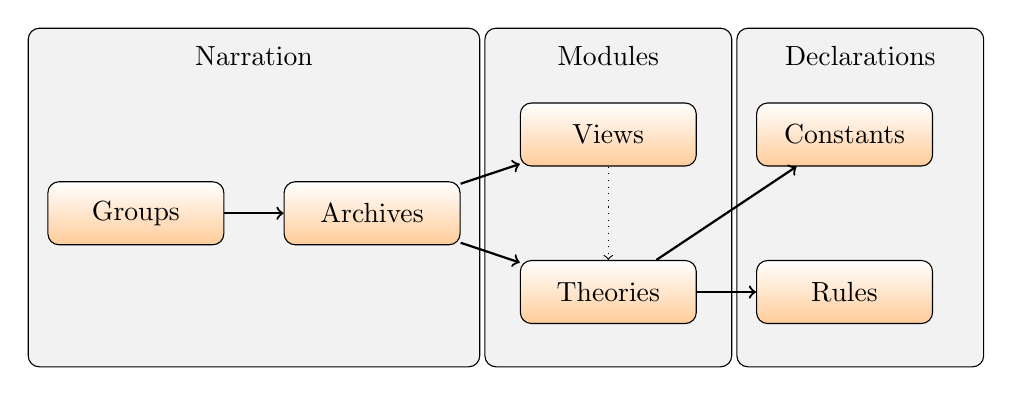
\begin{tikzpicture}[xscale=\myxscale, yscale=\myyscale]
  \tikzstyle{component} = [rectangle, draw, fill=orange!20, text width=2cm, text centered,
                                    rounded corners, minimum height=.8cm,shade,
                                    top color=white, bottom color=orange!40]
  \tikzstyle{back} = [rectangle, draw, fill=gray!10, text width=2cm,
                                    rounded corners, minimum height=4.3cm]
\node[back, text width = 5.5cm,  label ={[shift={(0ex,-4ex)}]north:Narration}] (nar) {};
\node[back, right of =nar, xshift=3.5cm, text width = 2.9cm,  label ={[shift={(0ex,-4ex)}]north:Modules}] (mod) {};
\node[back, right of =mod, xshift=2.2cm, text width = 2.9cm,  label ={[shift={(0ex,-4ex)}]north:Declarations}] (dec) {};
\node[component, left of =nar, xshift=-0.5cm, yshift=-0.2cm] (groups) {Groups};
\node[component, right of =groups, xshift=2cm] (archives) {Archives};
\node[component, right of =archives, xshift=2cm, yshift=-1cm] (theo) {Theories};
\node[component, right of =archives, xshift=2cm, yshift=1cm] (views) {Views};
\node[component, right of=theo, xshift=2cm, yshift=2cm] (con) {Constants};
\node[component, right of=theo, xshift=2cm] (rul) {Rules};
\draw[->, thick] (groups) -- node[above]{} (archives);
\draw[->,thick] (archives) -- node[above]{} (theo);
\draw[->,thick] (archives) -- node[above]{} (views);
\draw[->,thick] (theo) -- node[above]{} (rul);
\draw[->,thick] (theo) -- node[above]{} (con);
\draw[->,dotted] (views) -- node[above]{} (theo);
\end{tikzpicture}}
\caption{The MMT Structure}
\label{fig:mmt}
\end{figure}
To create a frontend that displays MMT it is important to get familiar with its structure, that can be seen in Figure \ref{fig:mmt}.
First up on the highest level are the individual groups.
Each group contains several archives.
An archive can be described as a collection of documents that typically are equivalent to a software project.
Therefore it provides a work flow for a language in MMT.
Groups and archives only exist to help the user to navigate through the library as well as to give a human readable description of the mathematical knowledge.
The modules that can be found in an archive, make up the actual content.
These are either theories or a view that shows the relation between multiple theories.
A theory is defined by its declarations which can be either rules or constants \cite{mmt}.

\subsection{MathHub} \label{mathhub}
MathHub.info is a portal specifically created for the active mathematical documents of MMT.
As stated before each one of these documents has a different degree of formal and informal content.
The representation of this data, knowledge and structure with varying degrees of formality is called \textbf{flexiformal} \cite{flexiforms}.
But realizing machine support for this approach of representing knowledge comes with a high formalization cost.
As a consequence it can be quiet challenging to find the right balance between costs and machine support.
The latest stable release of MathHub is available on \url{https://mathhub.info}.
The newest development of the system can be seen on \url{https://beta.mathhub.info}, but it is possible that some parts of this website do not work as intended. 

\subsection{Previous Implementation} \label{previous}
Since MathHub.info has been active for a couple of years there already exists a foundation for the system that can be adjusted to the new User Interface.
The previous realization can be seen in Figure \ref{fig:old_architecture}.
The source documents were stored, edited and converted on the GitLab repository manager.
There the documents are organized into their proper repositories and converted from their source formats into OMDoc/MMT.
These documents could be edited by their authors in a working copy of the GIT repository.
From there the MMT API could load the documents and send them to the frontend.
The frontend itself was implemented with \textbf{Drupal} \cite{comp}, while user interactions were handled by the JavaScript modules in the JOBAD framework \cite{jobad}.
Drupal is an open source content-management framework that also supplies uniform theming and is currently used by millions of different websites.
The reason Drupal was used for the User Interface up until April 2018 was that it has an integrated rights-management.
\begin{figure}[H]
  \begin{tikzpicture}[xscale=\myxscale,yscale=\myyscale]
    \tikzstyle{system} = [rectangle, draw, fill=orange!20, text width=1cm, text centered,
                                      rounded corners, minimum height=.8cm,shade, 
                                      top color=white, bottom color=orange!20]
     \tikzstyle{database} = [rectangle, draw, fill=blue!20, text width=1.3cm, text centered,
                                      rounded corners, minimum height=.8cm,shade, 
                                      top color=white, bottom color=blue!20] 
  \node[inner sep=0pt] (user) at (0,0){
\includegraphics[width=.1\textwidth]{user.png}};
  \node[system,right of =user,text width=1.7cm, xshift=2.7cm] (browser) {Browser}; 
  \node[system,right of= browser,text width=1.7cm, xshift=2.6cm] (drupal) {Drupal};
  \node[system,above right of =drupal, xshift = 2.8cm] (mmt) {MMT};
  \node[system,below right of =drupal, xshift = 2.8cm, text width=1.2cm] (gl) {GitLab};
  \node[database,below left of =gl, yshift = -0.6cm, xshift = -3cm] (lib) {library};
  \node[inner sep=0pt, below right of =gl, yshift = -0.6cm, xshift = 1.6cm] (author) {
\includegraphics[width=.1\textwidth]{author.jpg}}; 
  \node[below right of =mmt, yshift =0.7cm,  xshift = 1.6cm] (conv) {\begin{tabular}{l}\footnotesize convert to\\ OMDoc\\/MMT\end{tabular}};
  \node[above of=browser, yshift=0.25cm] (jobad){JOBAD};
  \draw[<-,thick] (mmt) -- node[left]{load} (gl);
  \draw[<->,dotted] (user) -- node[above]{read} node[below]{interact} (browser);
  \draw[<->,thick] (browser) -- node[above]{REST} (drupal);
  \draw[->,thick] (gl) to[loop left,out=20,in=45,looseness=11] (gl); 
  \draw[<->,dashed] (conv) -- (mmt);
  \draw[<->, dotted] (jobad) -- (mmt);
  \draw[<-,thick] (drupal) -- node[above]{present}(mmt); 
  \draw[->,thick] (drupal) -- node[above]{edit}(gl); 
  \draw[->,dotted] (author) -- node[above, xshift=0.2cm]{local} node[below]{edit} (gl);
  \draw[->,dotted] (lib) -- node[below, yshift=-0.1cm]{import} (gl);
  \draw[->,thick] (browser) to [loop above] ();
  \end{tikzpicture}
  \caption{Old MathHub Architecture}
  \label{fig:old_architecture}
  \end{figure}
Initially it sounded like a good idea to have the user rights handled directly by the frontend.
But with time it showed that it is easier to use the rights-manager provided by GitLab.
In the end the users of Mathhub.info still had to deal with the huge overhead that is necessary to use Drupal without benefiting from its features.
This created a lot of unnecessary and tedious extra work.	

\subsection{Security Issues} \label{security}
Additionally a critical security flaw in the Drupal versions 6 to 8 went public in April 2018.
The problem is that these versions accept request parameters without any validation.
This means it processes any input from anybody \cite{zdnet}.
To exploit this weakness an attacker doesn't even need to log in or have any other privileges on a vulnerable website \cite{register}.
With this flaw it is possible to inject malicious code and compromise a website in multiple ways.
This can be used to access, change and delete private data and create backdoors to make future attacks possible.
The Drupal community called this weakness "Drupalgeddon2" while its official name was "CVE-2018-7600".
Some code that was injected installed the program XMRig Monero miner, which is a cryptocurrency mining program, as well as deleted other mining programs on the compromised system \cite{hacker}.
The National Institute of Standards and Technology (NIST) gave Drupal a "Highly Critical" rating because of this vulnerability \cite{nist}.
After this flaw was discovered a patch was published and a warning to update every website that used a vulnerable version was given.
\newline \newline	
Since there have been multiple security flaws in Drupal before that compromised MathHub.info, the decision was made to stop using it and rebuild the frontend from ground up with a lighter and easier to use framework to not be affected by future attacks.

\subsection{State of the art - Building an interactive Frontend} \label{SoA}
The first step of creating a new frontend is to chose a new framework.
There are many options available so lets take a look at the most popular ones in order to find the one that fits MathHub.info the best.
\newline \newline
\textbf{Polymer} \cite{polymer} is an open source JavaScript library developed and maintained by Google.
It uses the native technologies of a browser instead of large custom JavaScript libraries.
This makes Polymer remarkably fast on Chrome and Safari.
It also provides a set of features that makes it easy to create custom elements, that work like standard web components.
It is used for several Google services like Youtube, Google Earth, Google Play Music etc. as well as for the websites of Netflix, Electronic Arts and many other companies. 
\newline \newline
Another open source web framework from Google is \textbf{Angular} \cite{angular}.
This TypeScript library has a framework architecture that simplifies the development of new web applications.
Angular transfers all content of a website at once and leaves the task of building the page to the browser.
This significantly speeds up the loading process and search optimization while keeping the communication with the server at a minimum. 
It also has Angular Material, a collection of UI components that work in browsers, on mobile and desktop.
\newline \newline
After using Angular on several Google projects, Evan You decided to create his own JavaScript framework called \textbf{Vue.js} \cite{vuewiki}.
Depending on the project it can be scaled between a framework and a library.
Vue.js separates its view layer library from its support libraries for complex applications, to create an easy approach to the framework.
It also automatically keeps track of the dependencies between components.
Therefore the system knows what exactly has to be rerendered when a page changed \cite{vuegit}.
\newline \newline
In the end the decision was made to use \textbf{React}, developed by Facebook.
React is a component based framework that uses a virtual DOM to avoid unnecessary rerendering.
It was chosen because the focus on reusable components makes it perfect for a large and still growing system like MathHub.
Further details about React and how it is used can be found in Section \ref{react} and Section \ref{components}.

\subsection{The core concept of React} \label{react}
React \cite{reactjs} is an open source JavaScript library owned and maintained by Facebook.
It was created to build interactive user interfaces (UI), for example Facebook and Instagram.
What makes React unique is its use of a virtual Document Object Model (DOM).
The concept of the virtual DOM is that updating a website does not rerender everything.
React computes the differences between the last and the next page and only changes the necessary parts.
On top of that it also has conditional rendering which means that an item will only be rendered if it is shown.
The advantage of the virtual DOM and conditional rendering is that this makes updating a website fast, but it comes with high RAM costs.
The actual interface that is displayed in the browser is made up of many different elements and components.
A website that uses React can have multiple unique features so it is helpful to build new components to implement these features.
Further details on how to create components are discussed in Section \ref{components}.
\newline \newline
Since React was designed by Facebook, there was a need for a design pattern that handles a large code base better than MVC (Model View Controller).
This lead them to create an updated and improved version of the MVC and they named it \textbf{Flux}.
The philosophy behind the Flux design is that data flows only in one direction to create unidirectional cycles \cite{flux}.
\newline \newline
React itself does not have a styling system.
Consequently its community created the Semantic UI React library \cite{semantic} to provide an easy way to maintain a consistent theme throughout the frontend.
Of course it is still possible to use a different library or create new styling components but MathHub.info mostly uses Semantic UI React.

\subsection{Building new components in React} \label{components} 
This section provides insight into the work that takes up the majority of the time of creating, updating or amending to a part of the new MathHub.info frontend. 
The actual interface that can be seen in a browser is the combination of many individual components.
This way, on an update, the virtual DOM can check each component for differences.
As a result only the affected ones have to be rendered again.
\newline \newline
React already has large external libraries with a lot of different components, but it is often necessary to make new ones that have a desired functionality.
In JavaScript new components can either be implemented as a function or as a class.
Their inputs are called props.
To ensure the unidirectional design of React and prevent unwanted side effects in other components, props are read-only.
In addition to props each component can have an internal state.
Whenever a value in this state changes the component is rendered again.
Naturally a component can grow big rather quickly.
As it is possible to use components inside other components it is smart to split a big component into multiple smaller ones.
This has the advantage that components can be reused in many different locations with various purposes.
The actual output often has a tree structure with several levels.
\begin{figure}[H]
  \centerline{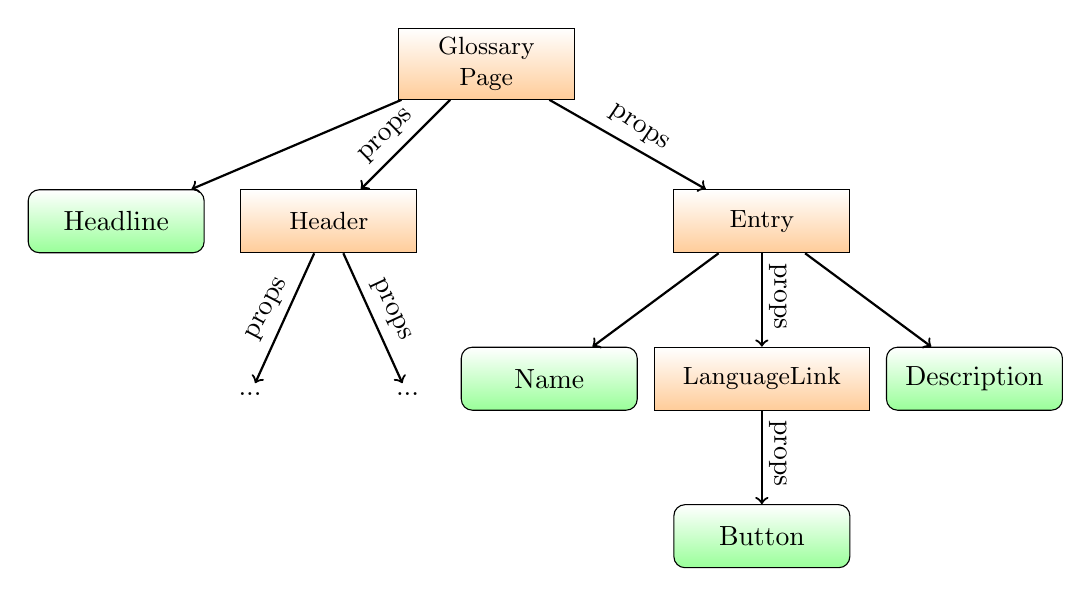
\begin{tikzpicture}[xscale=1, yscale=0.9]
    \tikzstyle{node} = [rectangle, draw, fill=orange!20, text width=2cm, yshift=-1cm, text centered,
                                      minimum height=.8cm,shade, font=\small,
                                      top color=white, bottom color=orange!40]
    \tikzstyle{leave} = [rectangle, draw, fill=green!20, text width=2cm, text centered, yshift=-1cm,
                                      rounded corners, minimum height=.8cm,shade, 
                                      top color=white, bottom color=green!40]
  \node[node](root){Glossary Page};
  \node[node, below of=root, xshift=-2cm](header){Header};
  \node[leave, below of=root, xshift=-4.7cm](headline){Headline};
  \node[node, below of=root, xshift=3.5cm](entry){Entry};
  \node[rectangle, yshift=-1.2cm, xshift=-1cm, below of=header](dots1){...};
  \node[rectangle, yshift=-1.2cm, xshift=1cm, below of=header](dots2){...};
  \node[leave, below of= entry, xshift=-2.7cm](name){Name};
  \node[node, below of=entry, text width=2.5cm](link){LanguageLink};
  \node[leave, below of=entry, xshift=2.7cm](desc){Description};
  \node[leave, below of=link](button){Button};
  \draw[->, thick] (root) -- node[above, rotate=44, xshift=-0.1cm]{props} (header);
  \draw[->, thick] (root) -- (headline);
  \draw[->, thick] (root) -- node[above, rotate=326]{props} (entry);
  \draw[->, thick] (header) -- node[above, rotate=62]{props} (dots1);
  \draw[->, thick] (header) -- node[above, rotate=295]{props} (dots2);
  \draw[->, thick] (entry) -- (name);
  \draw[->, thick] (entry) -- node[right, xshift=0.2cm, yshift=0.6cm, rotate=270]{props} (link);
  \draw[->, thick] (entry) -- (desc);
  \draw[->, thick] (link) -- node[right, xshift=0.2cm, yshift=0.6cm, rotate=270]{props} (button);
  \end{tikzpicture}}
  \caption{The React Component Tree of the Glossary Page}
  \label{fig:glossaryTree}
  \end{figure}
In this tree the nodes are the individual components and the leaves are the elements that are directly rendered by the DOM.
A good example for a tree with multiple levels is the Glossary Page of MathHub.info (more details about the Glossary can be found in Section \ref{routes} and \ref{gloss}), which can be seen in Figure \ref{fig:glossaryTree}.
In this example the headline can be rendered directly while the Header and the Entries are the child components of the Glossary.
They both have their own elements and several layers of children, resulting in this tree structure.
\newline \newline
The unidirectional design of React has the consequence that an update of a component can only affect its children.
But sometimes it is necessary for a component to change something on a higher level in the tree.
In this case it is possible to "lift up" the state.
This means moving the value that initiates the change to the state of the higher node. 
This node then has to give it back to its child as a prop.
\begin{figure}[H]
  \centerline{
  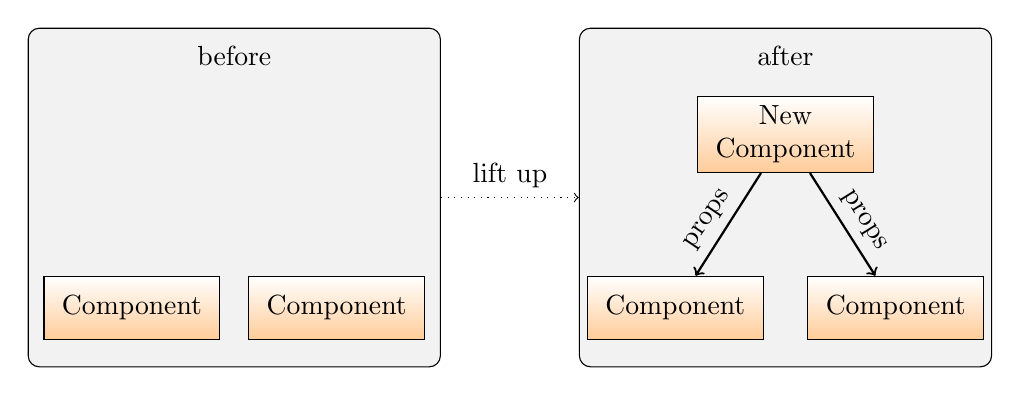
\begin{tikzpicture}[xscale=\myxscale, yscale=\myyscale]
    \tikzstyle{node} = [rectangle, draw, fill=orange!20, text width=2cm, text centered,
                                      minimum height=.8cm,shade, 
                                      top color=white, bottom color=orange!40]
                                      top color=white, bottom color=green!40]
    \tikzstyle{back} = [rectangle, draw, fill=gray!10, text width=5cm,
                                      rounded corners, minimum height=4.3cm]
  \node[back, label ={[shift={(0ex,-4ex)}]north:before}](oldb){};
  \node[node, below of=oldb, xshift=-1.3cm, yshift=-0.4cm](com1){Component};
  \node[node, right of=com1, xshift=1.6cm](com2){Component};
  \node[back, right of=oldb, xshift=6cm, label ={[shift={(0ex,-4ex)}]north:after}](newb){};
  \node[node, below of=newb, yshift=1.8cm](new){New Component};
  \node[node, below of=new, xshift=-1.4cm, yshift=-1.2cm](com3){Component};
  \node[node, below of=new, xshift=1.4cm, yshift=-1.2cm](com4){Component};
  \draw[->, thick] (new) -- node[above, rotate=56, xshift=-0.1cm]{props} (com3);
  \draw[->, thick] (new) -- node[above, rotate=302, xshift=0.1cm]{props} (com4);
  \draw[->, dotted] (oldb) -- node[above]{lift up} (newb);
  \end{tikzpicture}}
  \caption{Lifting up the State to a new Component}
  \label{fig:lift}
  \end{figure}
  Sometimes an update of a state should affect other components on the same level.
As shown in Figure \ref{fig:lift}, this can be done by lifting up the state to a new node that has all the components as children, that are affected by the update \cite{reactjsGS}.
The scalability and the ability to adapt to change of this design makes the React framework perfect for a mathematics information system like MathHub.info.
Creating new components and lifting up the state makes it easier to to add new functionalities and adjust the representation without creating the need to rebuild entire sections of the frontend.

\section{Realization} \label{architecture}
This Section gives a more in depth description of some parts of the implementation of the new MathHub system.
It starts with the updated Version of the architecture.
Next Section \ref{routes} introduces all Routes that currently exist in the frontend.
A Route leads to a specific page that is accessible on MathHub.info.
After that there is a brief outline of the communication between the backend and the frontend. 
The final part of Section presents the layout that is used for the entire User Interface.
\subsection{The Architecture of MathHub}
\begin{figure}[H]
  \begin{tikzpicture}[xscale=\myxscale,yscale=\myyscale]
  \tikzstyle{system} = [rectangle, draw, fill=orange!20, text width=1cm, text centered,
                                    rounded corners, minimum height=.8cm,shade, 
                                    top color=white, bottom color=orange!20]
   \tikzstyle{database} = [rectangle, draw, fill=blue!20, text width=1.3cm, text centered,
                                    rounded corners, minimum height=.8cm,shade, 
                                    top color=white, bottom color=blue!20] 
\node[inner sep=0pt] (user) at (0,0){
\includegraphics[width=.1\textwidth]{user.png}};
\node[system,right of =user,text width=1.7cm, xshift=2.7cm] (react) {React}; 
\node[system,right of= react,text width=2.6cm, xshift=2.6cm] (plugin) {MMT MathHub Plugin};
\node[system,above right of =plugin, xshift = 2.8cm] (mmt) {MMT};
\node[system,below right of =plugin, xshift = 2.8cm, text width=1.2cm] (gl) {GitLab};
\node[database,below left of =gl, yshift = -0.6cm, xshift = -3cm] (lib) {library};
\node[inner sep=0pt, below right of =gl, yshift = -0.6cm, xshift = 1.6cm] (author) {
\includegraphics[width=.1\textwidth]{author.jpg}}; 
\node[below right of =mmt, yshift =0.7cm,  xshift = 1.6cm] (conv) {\begin{tabular}{l}\footnotesize convert to\\ OMDoc\\/MMT\end{tabular}};
\draw[<-,thick] (mmt) -- node[left]{load} (gl);
\draw[<->,dotted] (user) -- node[above]{read} node[below]{interact} (react);
\draw[<->,thick] (react) -- node[above]{REST} (plugin);
\draw[->,thick] (gl) to[loop left,out=20,in=45,looseness=11] (gl); 
\draw[<->,dashed] (conv) -- (mmt);
\draw[<-,thick] (plugin) -- node[above]{present}(mmt); 
\draw[->,thick] (plugin) -- node[above]{edit}(gl); 
\draw[->,dotted] (author) -- node[above, xshift=0.2cm]{local} node[below]{edit} (gl);
\draw[->,dotted] (lib) -- node[below, yshift=-0.1cm]{import} (gl);
\end{tikzpicture}
\caption{New MathHub Architecture}
\label{fig:architecture}
\end{figure}
Now that a new framework has been chosen lets see how this changes the architecture of the MathHub system that was introduced in Section \ref{previous}.
The library is still stored and converted into OMDoc/MMT in GitLab.
But now the documents are loaded by a new plugin of an MMT server that provides the user with several semantic services in addition to the actual content.
The plugins responses to the requests of the React based frontend follow the constraints set by REST (Representational State Transfer) and use the JavaScript Object Notation (JSON).
The use of the Semantic-UI-React TypeScript library provides an universal theme throughout MathHub.info.
This results in the new architecture that is depicted in Figure \ref{fig:architecture}.
\newpage
\subsection{MathHub.info Routes} \label{routes}
To create a logical navigation system MathHub.info uses Routes to divide its content into numerous pages, that can be accessed from the \textbf{Homepage}.
The structure of these Routes can be seen in Figure \ref{fig:routes}.
\begin{figure}[H]
  \centerline{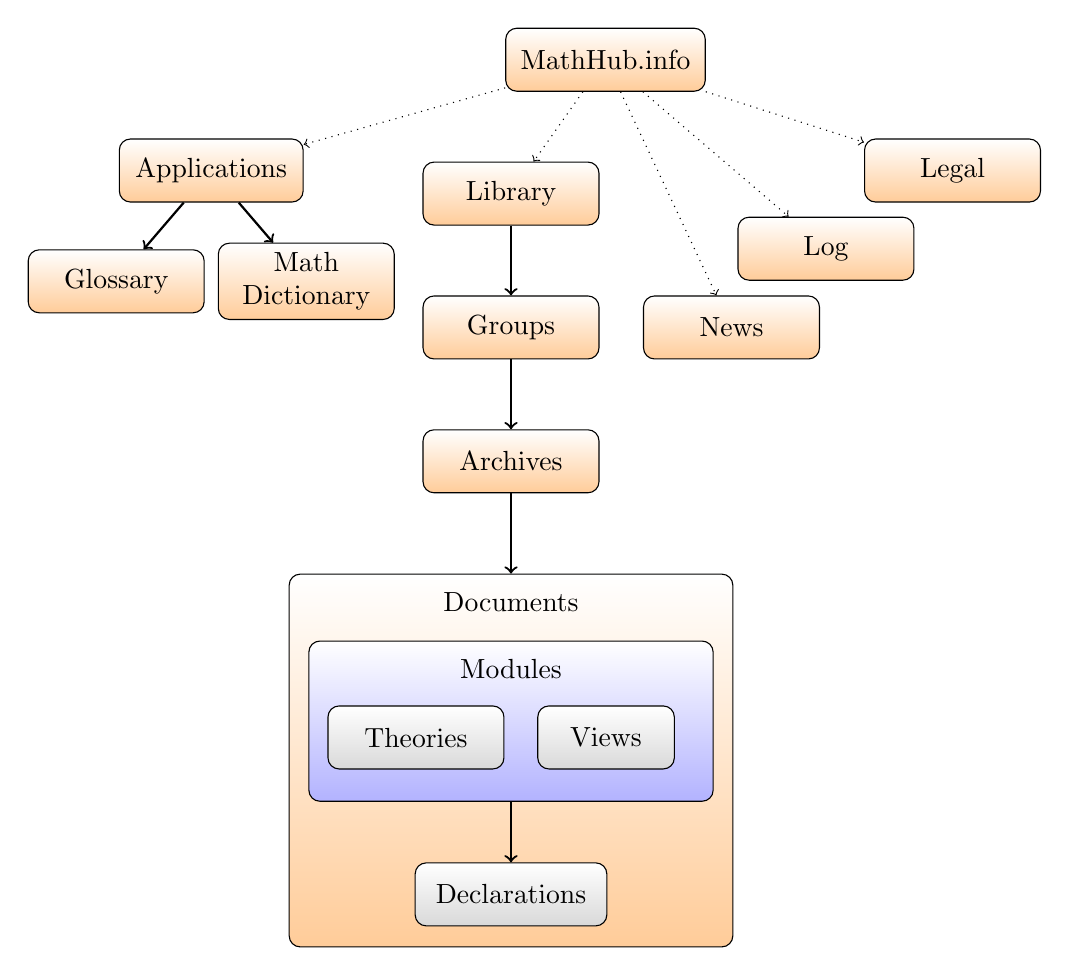
\begin{tikzpicture}[xscale=\myxscale, yscale=\myyscale]
    \tikzstyle{component} = [rectangle, draw, fill=orange!20, text width=2cm, text centered,
                                      rounded corners, minimum height=.8cm,shade, 
                                      top color=white, bottom color=orange!40]                                     
  \node[component, text width=2.3cm] (MH) {MathHub.info};
  \node[component, below of =MH, xshift=-1.2cm, yshift=-0.7cm] (lib) {Library};
  \node[component, below of =lib, yshift=-0.7cm] (groups) {Groups};
  \node[component, below of =groups, yshift=-0.7cm] (archives) {Archives};
  \node[component, below of =archives, text width=5.4cm, text height=4.5cm, yshift=-2.8cm, label ={[shift={(0ex,-4ex)}]north:Documents}] (doc) {};
  \node[component, below of =doc, text width=4.9cm, text height=1.8cm, yshift=1.5cm, label ={[shift={(0ex,-4ex)}]north:Modules}, bottom color=blue!30] (mod) {};
  \node[component, below left of =mod, xshift=-0.5cm, yshift=0.5cm, bottom color=black!15] (theo) {Theories};
  \node[component, below right of =mod, text width=1.5cm, xshift=0.5cm, yshift=0.5cm, bottom color=black!15] (views) {Views};
  \node[component, below of=mod, yshift=-1.2cm, text width=2.2cm, bottom color=black!15] (decl) {Declarations};
  \node[component, below left of =MH, xshift = -4.3cm, yshift=-0.7cm, text width=2.1cm] (apps) {Applications};
  \node[component, below left of =apps, xshift=-0.5cm, yshift=-0.7cm] (glos) {Glossary};
  \node[component, below right of =apps, xshift=0.5cm, yshift=-0.7cm] (dict) {Math Dictionary};
  \node[component, below of=MH, xshift=1.6cm, yshift=-2.4cm] (news) {News};
  \node[component, below of=MH, xshift=2.8cm, yshift=-1.4cm] (log) {Log};
  \node[component, below right of=MH, xshift=3.7cm, yshift=-0.7cm] (legal) {Legal};
  \draw[->,dotted] (MH) -- node[above]{} (lib);
  \draw[->,dotted] (MH) -- node[above]{} (apps);
  \draw[->,dotted] (MH) -- node[above]{} (news);
  \draw[->,dotted] (MH) -- node[above]{} (log);
  \draw[->,dotted] (MH) -- node[above]{} (legal);
  \draw[->,thick] (lib) -- node[above]{} (groups);
  \draw[->, thick] (groups) -- node[above]{} (archives);
  \draw[->,thick] (archives) -- node[above]{} (doc);
  \draw [->,thick] (mod) -- node[above]{} (decl);
  \draw[->,thick] (apps) -- node[above]{} (glos);
  \draw[->,thick] (apps) -- node[above]{} (dict);
  \end{tikzpicture}}
  \caption{MathHub Routes}
  \label{fig:routes}
  \end{figure}  
First of is the main content of MathHub, the \textbf{MMT Library}.
It starts with the different \textbf{Groups}.
The next page displays the \textbf{Archives} that belong to a specific group.
Groups and archives exist only for narration and navigation purposes.
This means they don't have any actual content only meta information like names and descriptions.
The actual content can be found in the \textbf{Documents}.
These documents consist of multiple modules (i.e. theories and views) as well as opaque elements that give the user additional information about the theories.
The archive-page has a list of all the documents in an archive.
On the document-page the user can find modules with all their declarations.
\newline \newline
The many groups, archives and theories within the MathHub library make use of a lot of mathematical terms.
In addition to being a collection of these expressions, the \textbf{Glossary} also provides a definition for each term.
Over the time many different authors have contributed to the MathHub library, therefore it can happen that there are different terms that share the same meaning.
These synonyms can also be found in the Glossary.
Since many theories exist in multiple languages it makes sense to have a Glossary available for every used language.
Currently the biggest collection of terms are in the English Glossary, followed by German and French.
Smaller collections for Turkish and Romanian are also available as well as simplified and traditional Chinese \cite{smglom}.
\newline \newline
Most of the times a user does not want to browse through the gigantic Glossary just to find a single term.
This is the reason why the \textbf{Math Dictionary} is a useful extension of the Glossary.
The main purpose of the Math Dictionary is to translate a term into another language and look up a definition of a specific expression.
\newline \newline
There is also a page with all the latest \textbf{News} regarding MathHub, as well as a couple of static pages like \textbf{Licenses} and the \textbf{Privacy Policy}.
At last there is a \textbf{Log} for the developers that shows the most recent messages from the backend.

\subsection{Communication with the Backend}
As previously mentioned the frontend does not have any actual content.
It gets the data from the MMT backend.
MathHub.info has several clients that each communicate with a part of the server when their specific functionality is needed.
The different clients are:
\begin{itemize}
\item a Library Client for everything related to the content of the library
\item a Glossary Client that gets all the terms in a specific language
\item a Translation Client that is used by the Math Dictionary to search for a translation of a term 
\item a News Client
\item a Log Client
\end{itemize}
The answers that are received from the backend use the JSON format.
The data objects in JSON consist of attribute-value pairs and arrays.
The frontend then uses these objects as props for React components.
\newpage
\subsection{Layout}
Every page consists of three parts: A header, a footer and the actual content in between.
This is illustrated with the Homepage as an example in Figure \ref{fig:home}.
\begin{figure}[H]
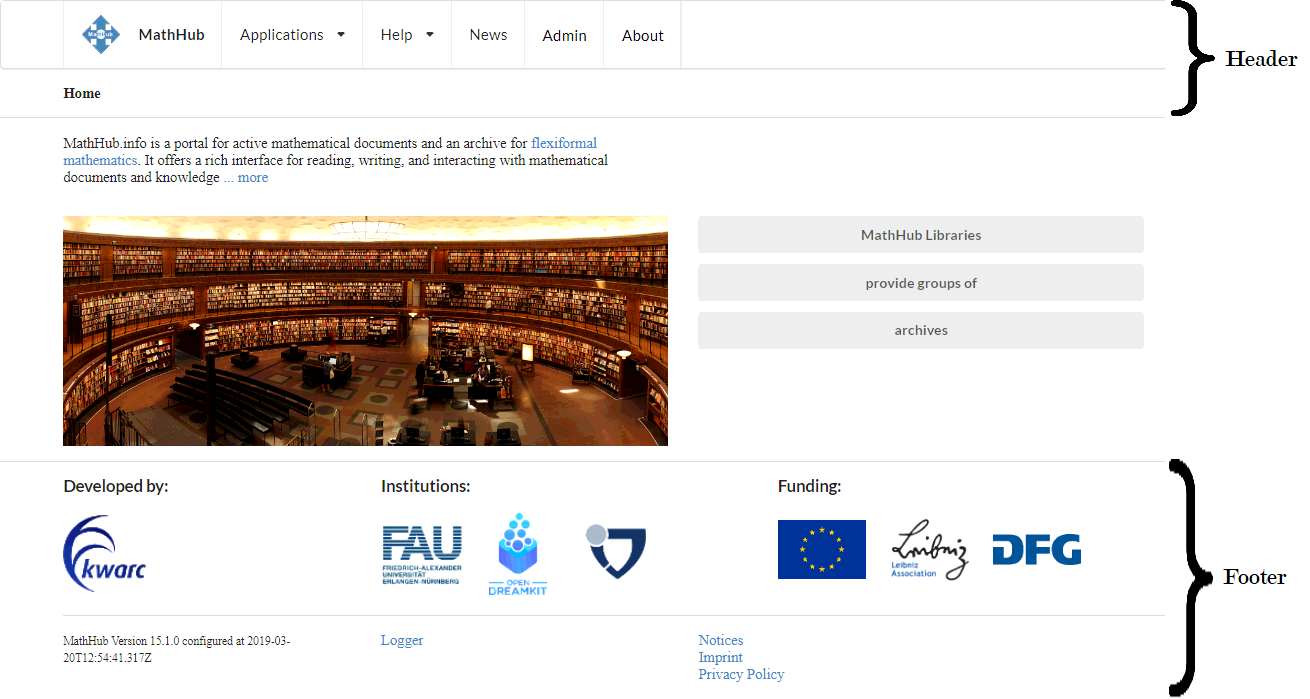
\includegraphics[width=1\textwidth]{home2.png}
\caption{The Homepage}
\label{fig:home}
\end{figure}
The header is a menu with the Routes to Home, the News, the Glossary and the Math Dictionary as well some external links.
Under the menu there are breadcrumbs that help the user to navigate through the library.
\newline \newline
The logos of the institutions that are involved in MathHub as well as the Routes that are used less commonly can be found in the footer.
These lead to the log, the licenses, the imprint and the privacy policy.
All these Routes and links are independent from the current page.
Therefore they should always be accessible.
The body that is displayed in between depends on the content of the present page.
\newpage
\section{MathHub Library Components} \label{library}
This Section discusses the design choices for the different components of the MathHub library.
Each page tries to maintain a certain degree of clarity while giving enough information about the currently displayed content to the user.
The challenge to find the right balance results in a very clean theme throughout the library.
The first page of the library can be seen in Figure \ref{fig:lib}.
It has a list of all the groups of MathHub.
Every group is rendered as its own React component that has the name of the group, a short teaser and links to the corresponding group-page.
\begin{figure}[H]
  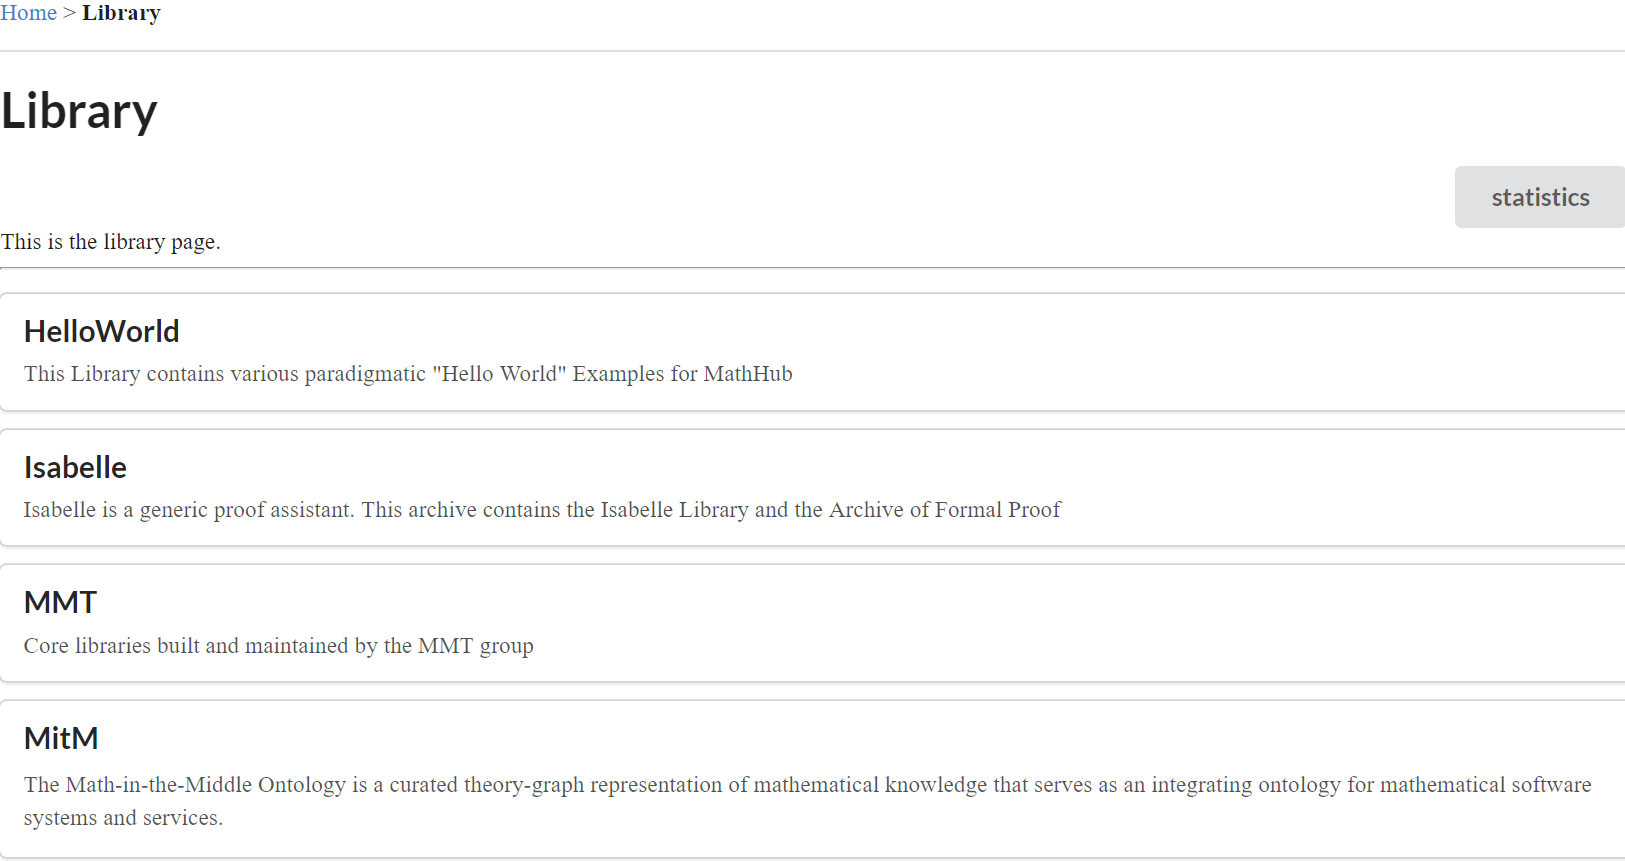
\includegraphics[width=1\textwidth]{library.png}
  \caption{The MathHub Library in the Frontend}
  \label{fig:lib}
\end{figure}
  
\subsection{Groups}
\begin{figure}[H]
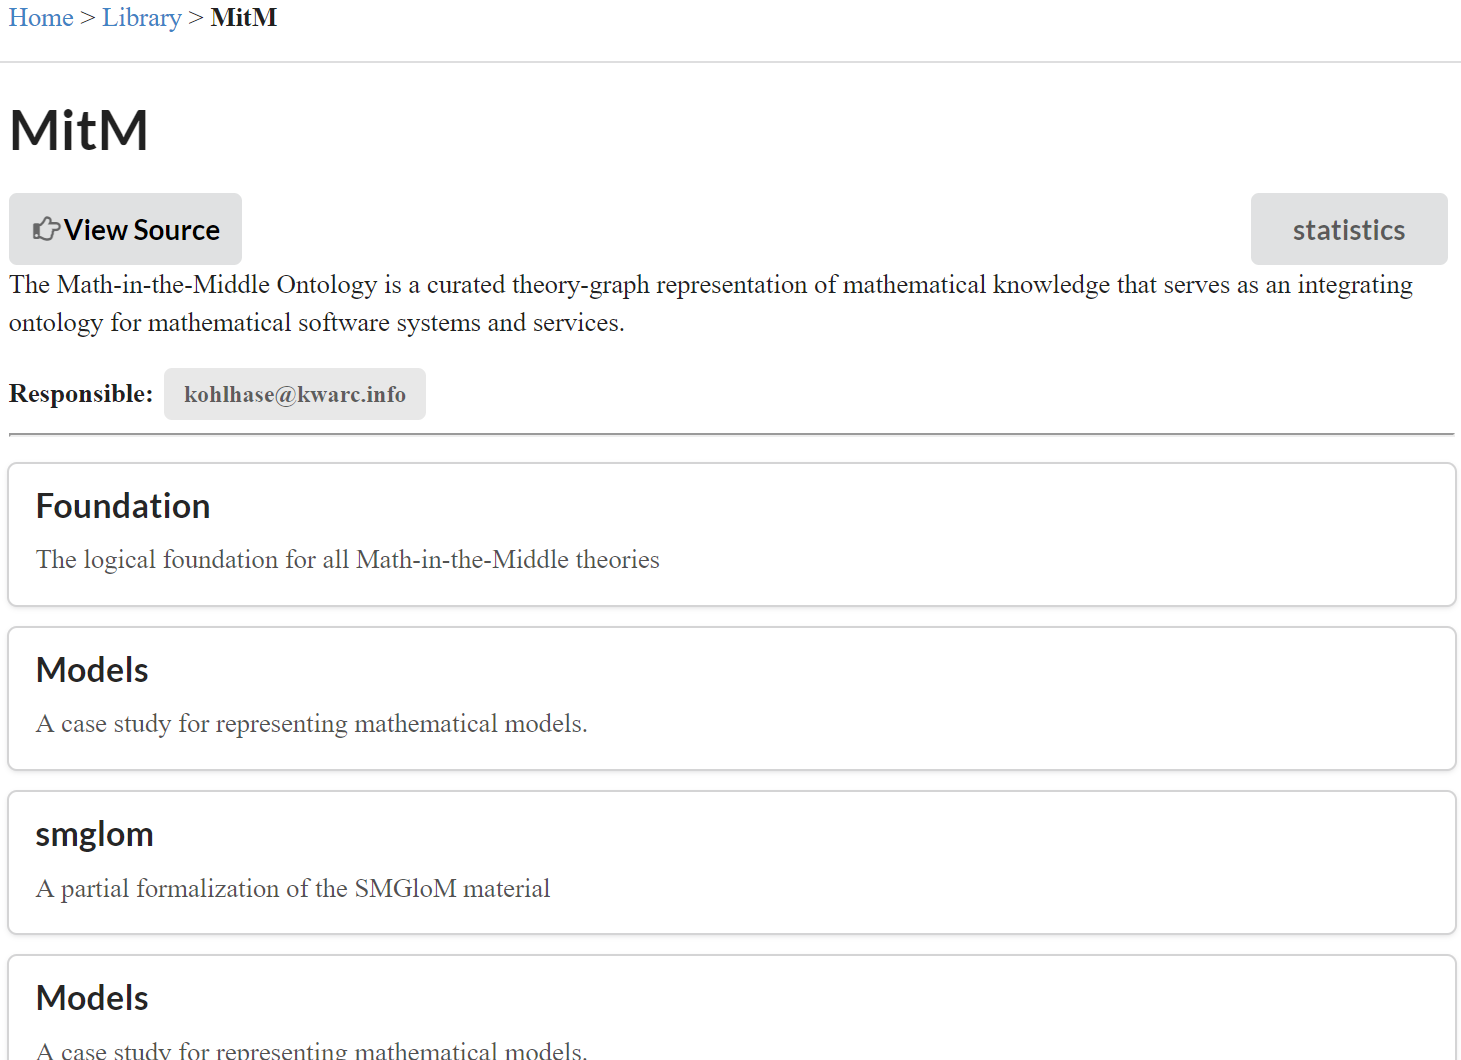
\includegraphics[width=1\textwidth]{group.png}
\caption{A Group in the Frontend}
\label{fig:group}
\end{figure}
As an example Figure \ref{fig:group} shows a screenshot of the MitM group as it is depicted on MathHub.info.
Above the numerous archives the group page starts with a header that has the same structure for every group.
It begins with a button that links to its source files on GitLab.
After that follows a description that gives an overview of the groups content.
The header ends with a list of e-mail addresses of the people that maintain the group.
\newline \newline
Beneath that there is a list of all the corresponding archives.
Every archive is its own React component that consists of a name and a short teaser that summarizes its content for the user.
By clicking on an entry the user is taken to the corresponding archive-page.
The overall design of the group-page is very similar to library-page because the entries of the list of each site have a teaser that provides a bit more information than just the name.
This consistency helps the user to quickly get adjusted to the UI.
Additionally a slightly different design was tested, but having two list entries per row greatly decreased the overview of the page.
Therefore the choice was made that each row only has one entry that takes up the entire width.

\subsection{Archives}
\begin{figure}[H]
\centerline{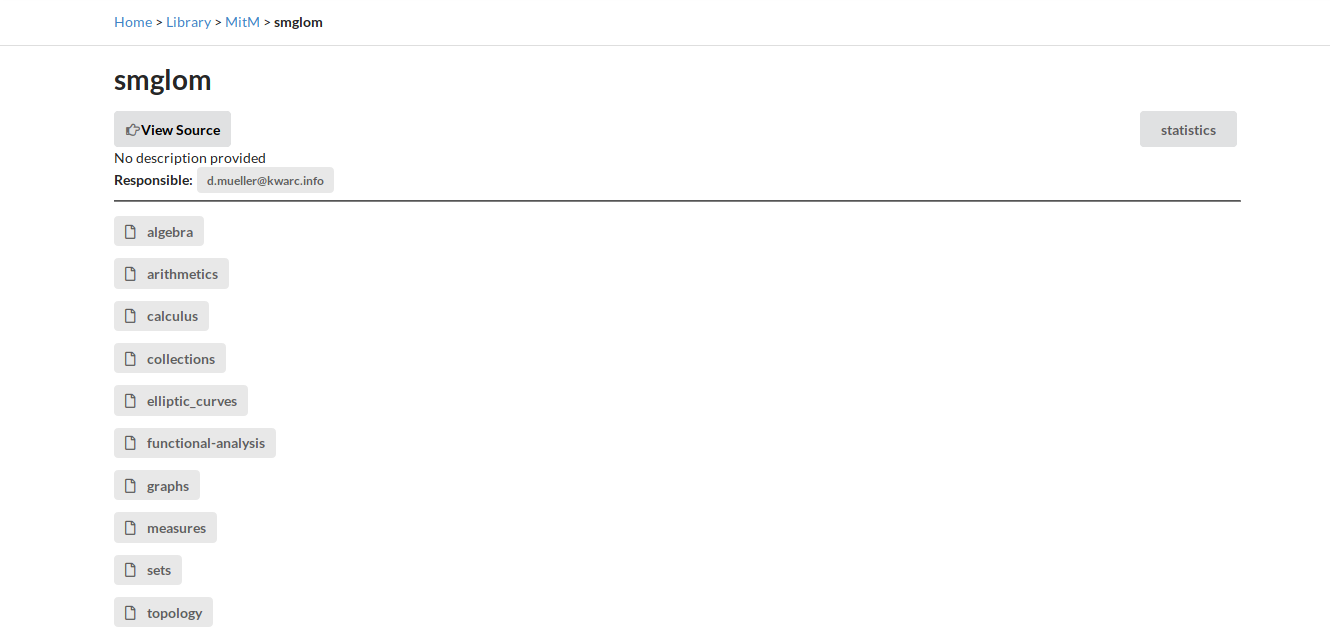
\includegraphics[width=0.4\textwidth]{archive.png}}
\caption{An Archive in the Frontend}
\label{fig:archive}
\end{figure}
Figure \ref{fig:archive} shows that the structure of the archive-page is very similar to the group-page.
It also starts with a header that consists of a button that links to the source files, a description of the archive and the e-mail addresses of the responsible people. 
\newline \newline
After the header follows a list of the documents in that archive.
There is the main difference between the group-page and the archive page.
Currently the document entries do not have a teaser text.
As a result they just link to the document-page and do not need to take up the entire width.
But sometimes the names do not give much information about the content of the document.
Therefore it would be advantageous to add short teaser.
Then the design of the list entries should be changed to be like the lists of the group- and library-page.

\subsection{Documents}
\begin{figure}[H]
\centerline{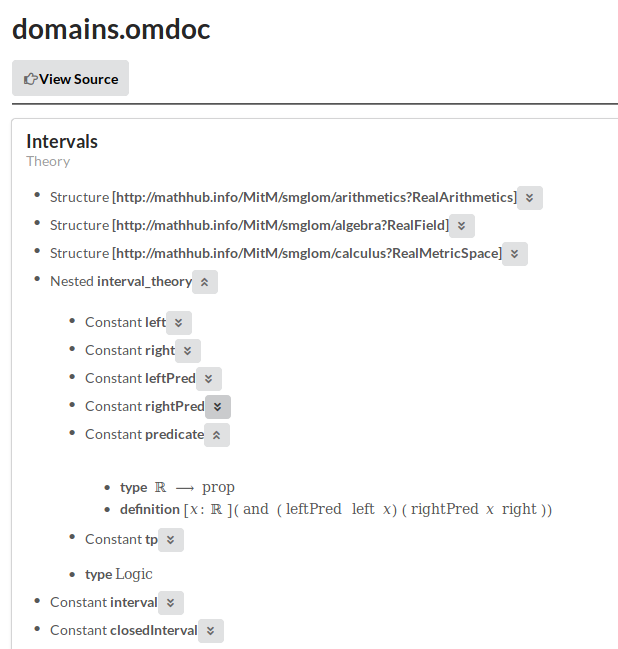
\includegraphics[width=0.8\textwidth]{document.png}}
\caption{A Document in the Frontend}
\label{fig:doc}
\end{figure}
Depending on the document, its page can be a combination of modules and opaque elements as well as links to further documents.
Figure \ref{fig:doc} displays a document in the OMDoc format.
There is also a button that links to a documents source file on GitLab.
\newline \newline
The modules are expandable React components that consist of a name, a type, either theory or view and a button to show further details.
Clicking on the button shows all the declarations and nested theories inside of that module.
These declarations (structure elements, constants, rule constants etc.) and theories can be further extended to show their own content.
Some documents can have a great number of declarations.
Therefore it would take a lot time to load every single one from the MMT server.
They are hidden at first to make the document available faster.
When the user clicks the button to make the declarations visible, the frontend sends a new request to the backend. 
\newline \newline
In between the modules there can be opaque elements.
Opaque elements are just text that help the user to understand or give some additional information about the document.
These make up the informal part of theories in MMT.

\subsection{Statistics}
\begin{figure}[H]
\centerline{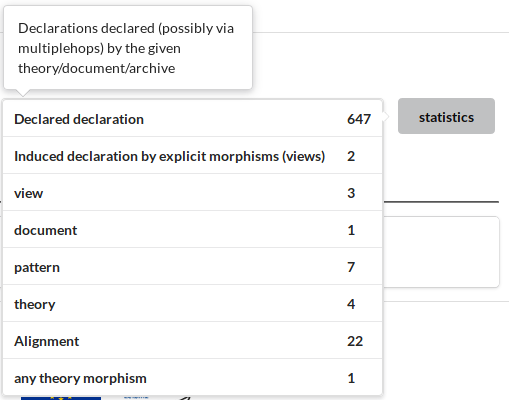
\includegraphics[width=0.6\textwidth]{statistics.png}}
\caption{Statistics in the Frontend}
\label{fig:stats}
\end{figure}
On every group-, archive- and document-page there also is a statistics button that shows some available statistics about that particular group, archive or document.
When the cursor hovers over a keyword of a statistic that keyword is explained in a pop-up as can be seen in Figure \ref{fig:stats}.
\newpage
\section{The Applications of MathHub} \label{apps}
Now that the implementation of every level of the MathHub library has been show it is time to take a look at the pages of the Glossary and the Math Dictionary. 
Since these do not have a clear hierarchy structure like the library, they do need a different design approach.
\subsection{Glossary} \label{gloss}
\begin{figure}[H]
\includegraphics[width=1\textwidth]{glossary.png}
\caption{The Glossary in the Frontend}
\label{fig:glossary}
\end{figure}
As shown in Figure \ref{fig:glossary}, the glossary-page has a tab for every available language of the Glossary.
At any given time only the terms are rendered that have an entry in the currently selected language.
Additionally the Glossary shows the other languages for each term.
Thus there are two possible ways to change languages.
First by changing the language tab and second by clicking on a language-button inside an entry.
\newline \newline
To create a better overview the definition of a term is not immediately shown.
By clicking on an entry its definition and its synonyms become visible.

\subsection{Math Dictionary}
\begin{figure}[H]
\centerline{\includegraphics[width=0.7\textwidth]{dictionary.png}}
\caption{The Math Dictionary in the Frontend}
\label{fig:dict}
\end{figure}
Figure \ref{fig:dict} depicts the Math Dictionary of MathHub.info.
To translate a term with the help of the Math Dictionary the user has to select the current language of the term from a dropdown menu and also the language to which it should be translated into.
Pressing the "translate" - button sends a translation request to the MMT server.
Until the servers responds, the message "translating" is shown and the button is disabled to prevent sending to many translation requests at once.
If a translation exists then the translated term, its definition and potential synonyms are shown and the button is enabled again.
By selecting the same language for "from" and "to" the Math Dictionary can also be used to get the definition for an expression without searching the glossary.

\section{Conclusion and Future Work} \label{conclusion}
This thesis showed that a light framework is definitely a valuable option for building an User Interface for a mathematics information system.
Since the UI is just a part of a bigger architecture that also includes a server backend and an external storage, it does not need features like user right management and versioned storage.
This partition greatly reduces the costs of working with MathHub compared to the previous implementation with Drupal.
The ability to easily introduce new features and the scalability of React makes it a remarkable choice for this frontend.
\newline \newline
Having an established hierarchy for every group as well as consistent theme ensures an intuitive navigation through the MathHub library in order to create an accessible user experience.
As stated before MathHub.info is an ever-growing system in terms of content and functionalities.
This reality in combination with new insight gained through continuous usage of the system will naturally lead to improvements made to the individual pages of the frontend.
As of right now the clean design introduced in this paper proved to be adequate.
\newline \newline
There already are plans to add certain features in the future. 
The biggest expansions that will be added to MathHub.info before long are TGView and MathWebSearch.

\subsection{TGView} 
TGView is a graph viewer with the task to visualize the relations between multiple theories to give a better overview over a system like MathHub.
The distinctive feature of TGView is that its backend sends all necessary data at once so every interaction can be handled by the frontend.
That means that its graphical interface is build on the client side to avoid sending a server request every time the user interacts with the interface, eg move or hide nodes.
Otherwise it would be required to refresh the page on every single change to the graph \cite{tgview}.
\newline \newline 
Even though the old MathHub frontend did have static graphs to show the relations between theories, it never integrated TGView.
 
\subsection{MathWebSearch}
Since MMT is a combination of formal and informal languages there is a need for a special search engine that can deal with this library.
The search engine that will be used within MathHub.info is called MathWebSearch \cite{HamKoh:fsfm15}.
It is able to search documents that have formulae of a certain shape.
For example searching the formula "?x+1" would return documents with formulae like "1+1", "x+1" etc. with that shape.
For Mathhub.info a combination of MathWebSearch and normal text search is needed.
This combination is called Themasearch and the goal is to make it possible to use it via the User Interface.

\subsection{Subset Frontend}
Currently MathHub.info is a place to showcase every MMT group.
But some of these groups could benefit from specialized additional features or a slightly different structure.
Therefore it makes sense to create subset frontends based on MathHub.info.
This way the subset frontends can be designed to perfectly fit their group without taking other groups into account.
In addition to new features they also should have a new Homepage to give the user a more detailed introduction than the short teaser that is shown on MathHub.info.
To summarize, the subset frontends will have a similar makeup as MathHub.info but will be adapted to better represent their content.

\subsection{Issue report: MathHub.info and content}
As of right now there is no direct way for a user to report an issue, a bug or request a new feature.
When this function is integrated into MathHub.info it would be appropriate to distinguish between two different kind of reports.

First, the user should be transferred to GitHub to open a new issue, if they have a problem with the frontend.

Second, if the user finds an issue within the content that is displayed on MathHub.info, they should be redirected to the corresponding GitLab page. 
\subsection{Jupyter Integration}
Recently the OpenDreamKit project has designed and implemented a Jupyter kernel \cite{notebook} for MMT. 
This kernel enables Jupyter to be used as a frontend for Math-in-the-Middle (MitM) operations.
Since MitM is part of the MathHub library it would make a great addition to integrate this feature into MathHub.info.
\newpage
\printbibliography
\end{document}